\section{Design Back-End}
\label{secD1:RequisitiBackEnd}

Nel presente capitolo vengono riportati i sistemi esterni con cui l'applicazione dovrà interfacciarsi per poter funzionare e una loro descrizione.

I sistemi esterni con cui PlanIt si dovrà interfacciare sono:
\begin{enumerate}
    \item sistemi di mappe: Google Maps e OpenStreetMap;
    \item sistema di gestione del calendario: Google Calendar;
    \item sistemi di pagamento: PayPal e/o Stripe;
    \item sistemi di autenticazione: Auth0;
    \item sistemi per la protezione da attacchi: Cloudflare;
    \item sistema di archiviazione delle informazioni: MongoDB;
    \item sistema di controllo della privacy e cookie: Iubenda.
          %\item sistema di posta elettronica: email.
\end{enumerate}

\subsection*{DESCRIZIONI}
\begin{listaPersonale}{BE}
    \elemento[Sistemi di mappe]{be:Mappe} Le API dei servizi di mappe Google Maps e OpenstreetMap, daranno la possibilità all'utente standard d'indicare la posizione esatta di dove si terrà l'impegno (\ref{rf:LuogoEvento}); tale posizione potrà essere specificata quando si compila il pop-up di compilazione impegno (\ref{rf:CreazioneModificaEvento}), oppure in un successivo momento durante la modifica dell'evento stesso (\ref{rf:CreazioneModificaEvento}).

    \elemento[Sistema di gestione del calendario]{be:Calendario} L'integrazione con Google Calendar (\ref{rf:GoogleCalendar}) permetterà d'importare ed esportare eventi dalla sua piattaforma.\\
    Il processo potrà avvenire mediante:
    \begin{itemize}
        \item L'importazione e l'esportazione tramite file: \\
              Si potranno importare ed esportare eventi da Google Calendar mediante l'utilizzo di un file.
        \item L'importazione e l'esportazione in automatico: \\
              Mediante l'uso delle API fornite dalla piattaforma Google Calendar, sarà possibile importare ed esportare eventi direttamente da e verso un calendario già esistente sulla piattaforma.
    \end{itemize}

    \elemento[Sistemi di pagamento]{be:Pagamento} L'integrazione con i sistemi di pagamento PayPal e Stripe gestiranno i pagamenti per la sottoscrizione a un account premium (\ref{rf:PagamentoUtentePremium}).

    \elemento[Sistema di autenticazione]{be:Autenticazione} Il sistema di autenticazione Auth0 gestirà la procedura di accesso e registrazione al sito (\ref{rf:AccessoRegistrazione}), permettendo accessi e registrazioni sicure (\ref{rnf:Sicurezza}) alla piattaforma. Mediante l'utilizzo di questo sistema di accesso esterno sarà anche possibile accedere e registrarsi direttamente sul sito tramite l'utilizzo di account di servizi terzi, tra cui: Google e altri eventuali servizi di terzi parti. \\ Infine, Auth0 gestisce completamente anche l'intera procedura del reset della password. Infatti, una volta inviato ad Auth0, da parte della piattaforma, la richiesta di recupero e reset della password, questo sistema esterno inizierà questa procedura richiedendo, all'inizio, l'email di recupero all'utente.

    \elemento[Sistemi per la protezione da attacchi]{be:Sicurezza} Il servizio CloudFlare verrà utilizzato per diversi scopi tra cui:
    \begin{enumerate}
        \item protezione da attacchi DDOS (\ref{rnf:Sicurezza});
        \item CDN (Content Delivery Network) in modo tale da servire le pagine statiche o file statici del sito con poca latenza;
        \item DNS così da poter creare diversi sotto domini;
        \item Certificato SSL, così da rendere sicura la connessione tra l'utente non autenticato e la piattaforma (\ref{rnf:Sicurezza}).
    \end{enumerate}

    \elemento[Sistema di archiviazione delle informazioni]{be:Database} Il sistema di archiviazione delle informazioni MongoDB dovrà gestire tutti i dati coinvolti nei processi della piattaforma, nello specifico: la memorizzazione del calendario, degli eventi, eventuali condivisioni, le informazioni di ogni utente standard per l'integrazione con i servizi di terze parti e le preferenze dell'utente standard.

    \elemento[Sistema di controllo della privacy e cookie]{be:PrivacyCookie} Il sistema di gestione della privacy e cookie Iubenda sarà utilizzato per generare una politica sulla privacy (\ref{rnf:Privacy}) che rispetterà i parametri di legge, e in caso di modifiche alle leggi in vigore informerà la piattaforma per adottare le modifiche necessarie per adempiere ai nuovi obblighi di legge. Inoltre Iubenda fornirà un' integrazione per accettare/rifiutare i cookie (\ref{rnf:Cookie}).

    \begin{comment}
    \elemento[Sistema di posta elettronica]{be:PostaElettronica} Il sistema di posta elettronica, email sarà utilizzato per inviare email informative sul sito ed email relative a comunicazioni per l'utente standard, ovvero:
    \begin{itemize}
        \item reset password (\ref{rf:RecuperoPassword});
        \item conferma creazione account (\ref{rf:AccessoRegistrazione});
        \item promemoria scadenza piano a pagamento (\ref{rf:UtentePremium}).
    \end{itemize}
    \end{comment}
\end{listaPersonale}

\subsection*{Servizi esterni}
\begin{center}
    \blfootnote{Immagine \href{https://github.com/Life-planner/Documentazione/blob/main/D1/img/Servizi/ServiziEsterni.drawio.png}{PNG}/\href{https://github.com/Life-planner/Documentazione/blob/main/D1/img/Servizi/ServiziEsterni.drawio.svg}{SVG}/\href{https://github.com/Life-planner/Documentazione/blob/main/D1/img/Servizi/ServiziEsterni.drawio.xml}{XML} servizi esterni}
    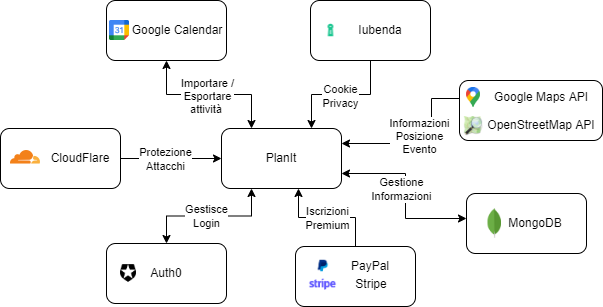
\includegraphics[width=1\textwidth]{img/Servizi/ServiziEsterni.drawio.png}
\end{center}